\section{Implementation}
\label{qoala:sec:implementation}
We implement our architecture in the form of an open-source simulator~\cite{qoala2023simulator}.
Implementation on real hardware requires developing new classical control hardware which is outside the scope of this work.
The simulator is built on top of NetSquid~\cite{coopmans2021netsquid} which can simulate quantum behavior as well as asynchronous classical processes.
Specifically, NetSquid provides detailed configuration allowing for simulations of hardware with parameters that are validated in real experiments, not possible using other simulators such as QuNetSim~\cite{diadamo2021qunetsim}, QNET~\cite{QNET}, and QuISP~\cite{satoh2022quisp}.
SquidASM~\cite{squidasmrepo} simulates the software and hardware stack used in the NetQASM/QNodeOS system mentioned in Section~\ref{qoala:sec:related_work}, and hence misses the scheduling capabilities that we introduce in Qoala.

The simulator has on purpose been made modular and composable:
components of Qoala's architecture (like CPS, QPS, scheduler, shared memory) are provided by the simulator as building blocks that can be configured and put together in different ways (details Appendix~\ref{qoala:sec:app:simulator}).
Both classical software parameters and quantum hardware noise models can be configured.
In this way, the simulator allows one to investigate different architecture and parameter choices.
% , and can therefore be used beyond just testing the Qoala architecture.
In the simulator, a network of quantum nodes implementing Qoala can be constructed, and Qoala programs can be submitted for execution to these nodes.
Static network schedules can be provided (capability negotiation and automatic network schedule creation are not simulated).
The simulator then executes the programs, providing application results and statistics.
% The simulator has also been used to perform our evaluation.
Our implementation allows researchers to not only test Qoala, but also configure parameters and architectures to investigate scheduling algorithms and hardware implementation choices.

\subsection{Scheduler implementation}
In our implementation, we use a two-level hierarchical scheduler architecture,
consisting of a node-wide \textit{node scheduler} which controls two \textit{processor schedulers}, one for the CPS and one for the QPS (Figure~\ref{qoala:fig:scheduler_impl}, details in Appendix~\ref{qoala:sec:app:scheduling_execution}).
Such an approach has been used in other contexts not related to quantum networks~\cite{polychronopoulos1991hierarchical, girkar1994hierarchical}.

Each scheduler maintains their own task graph.
The node scheduler task graph contains all tasks (CPS or QPS) that are to be executed.
Each processor scheduler task graph is a partial copy of the node scheduler task graph containing only the tasks that can be executed by its own processor.
Edges in the node scheduler graph between heterogeneous tasks (i.e. between CPS and QPS tasks) are represented in the partial processor graphs by an \texttt{external-dependencies} node attribute. 
When a processor scheduler finishes a task, it is removed from the task graph and a signal is sent to the node scheduler.
The node scheduler updates its own task graph accordingly, and may then add new tasks to the task graph of the processor scheduler.
Write conflicts on the processor task graphs are avoided since tasks can only be added by the node scheduler, and tasks can only be removed by the processor scheduler.

The processor schedulers support both a first-come-first-serve (FCFS) and an earliest-deadline-first (EDF)~\cite{silberschatz2006operating} scheduling mechanism.
In our evaluation (Section~\ref{qoala:sec:evaluation}), deadlines are used as \textit{soft deadlines}, i.e. there is no guarantee about meeting deadlines.

\begin{figure}% [ht]
    \centering
    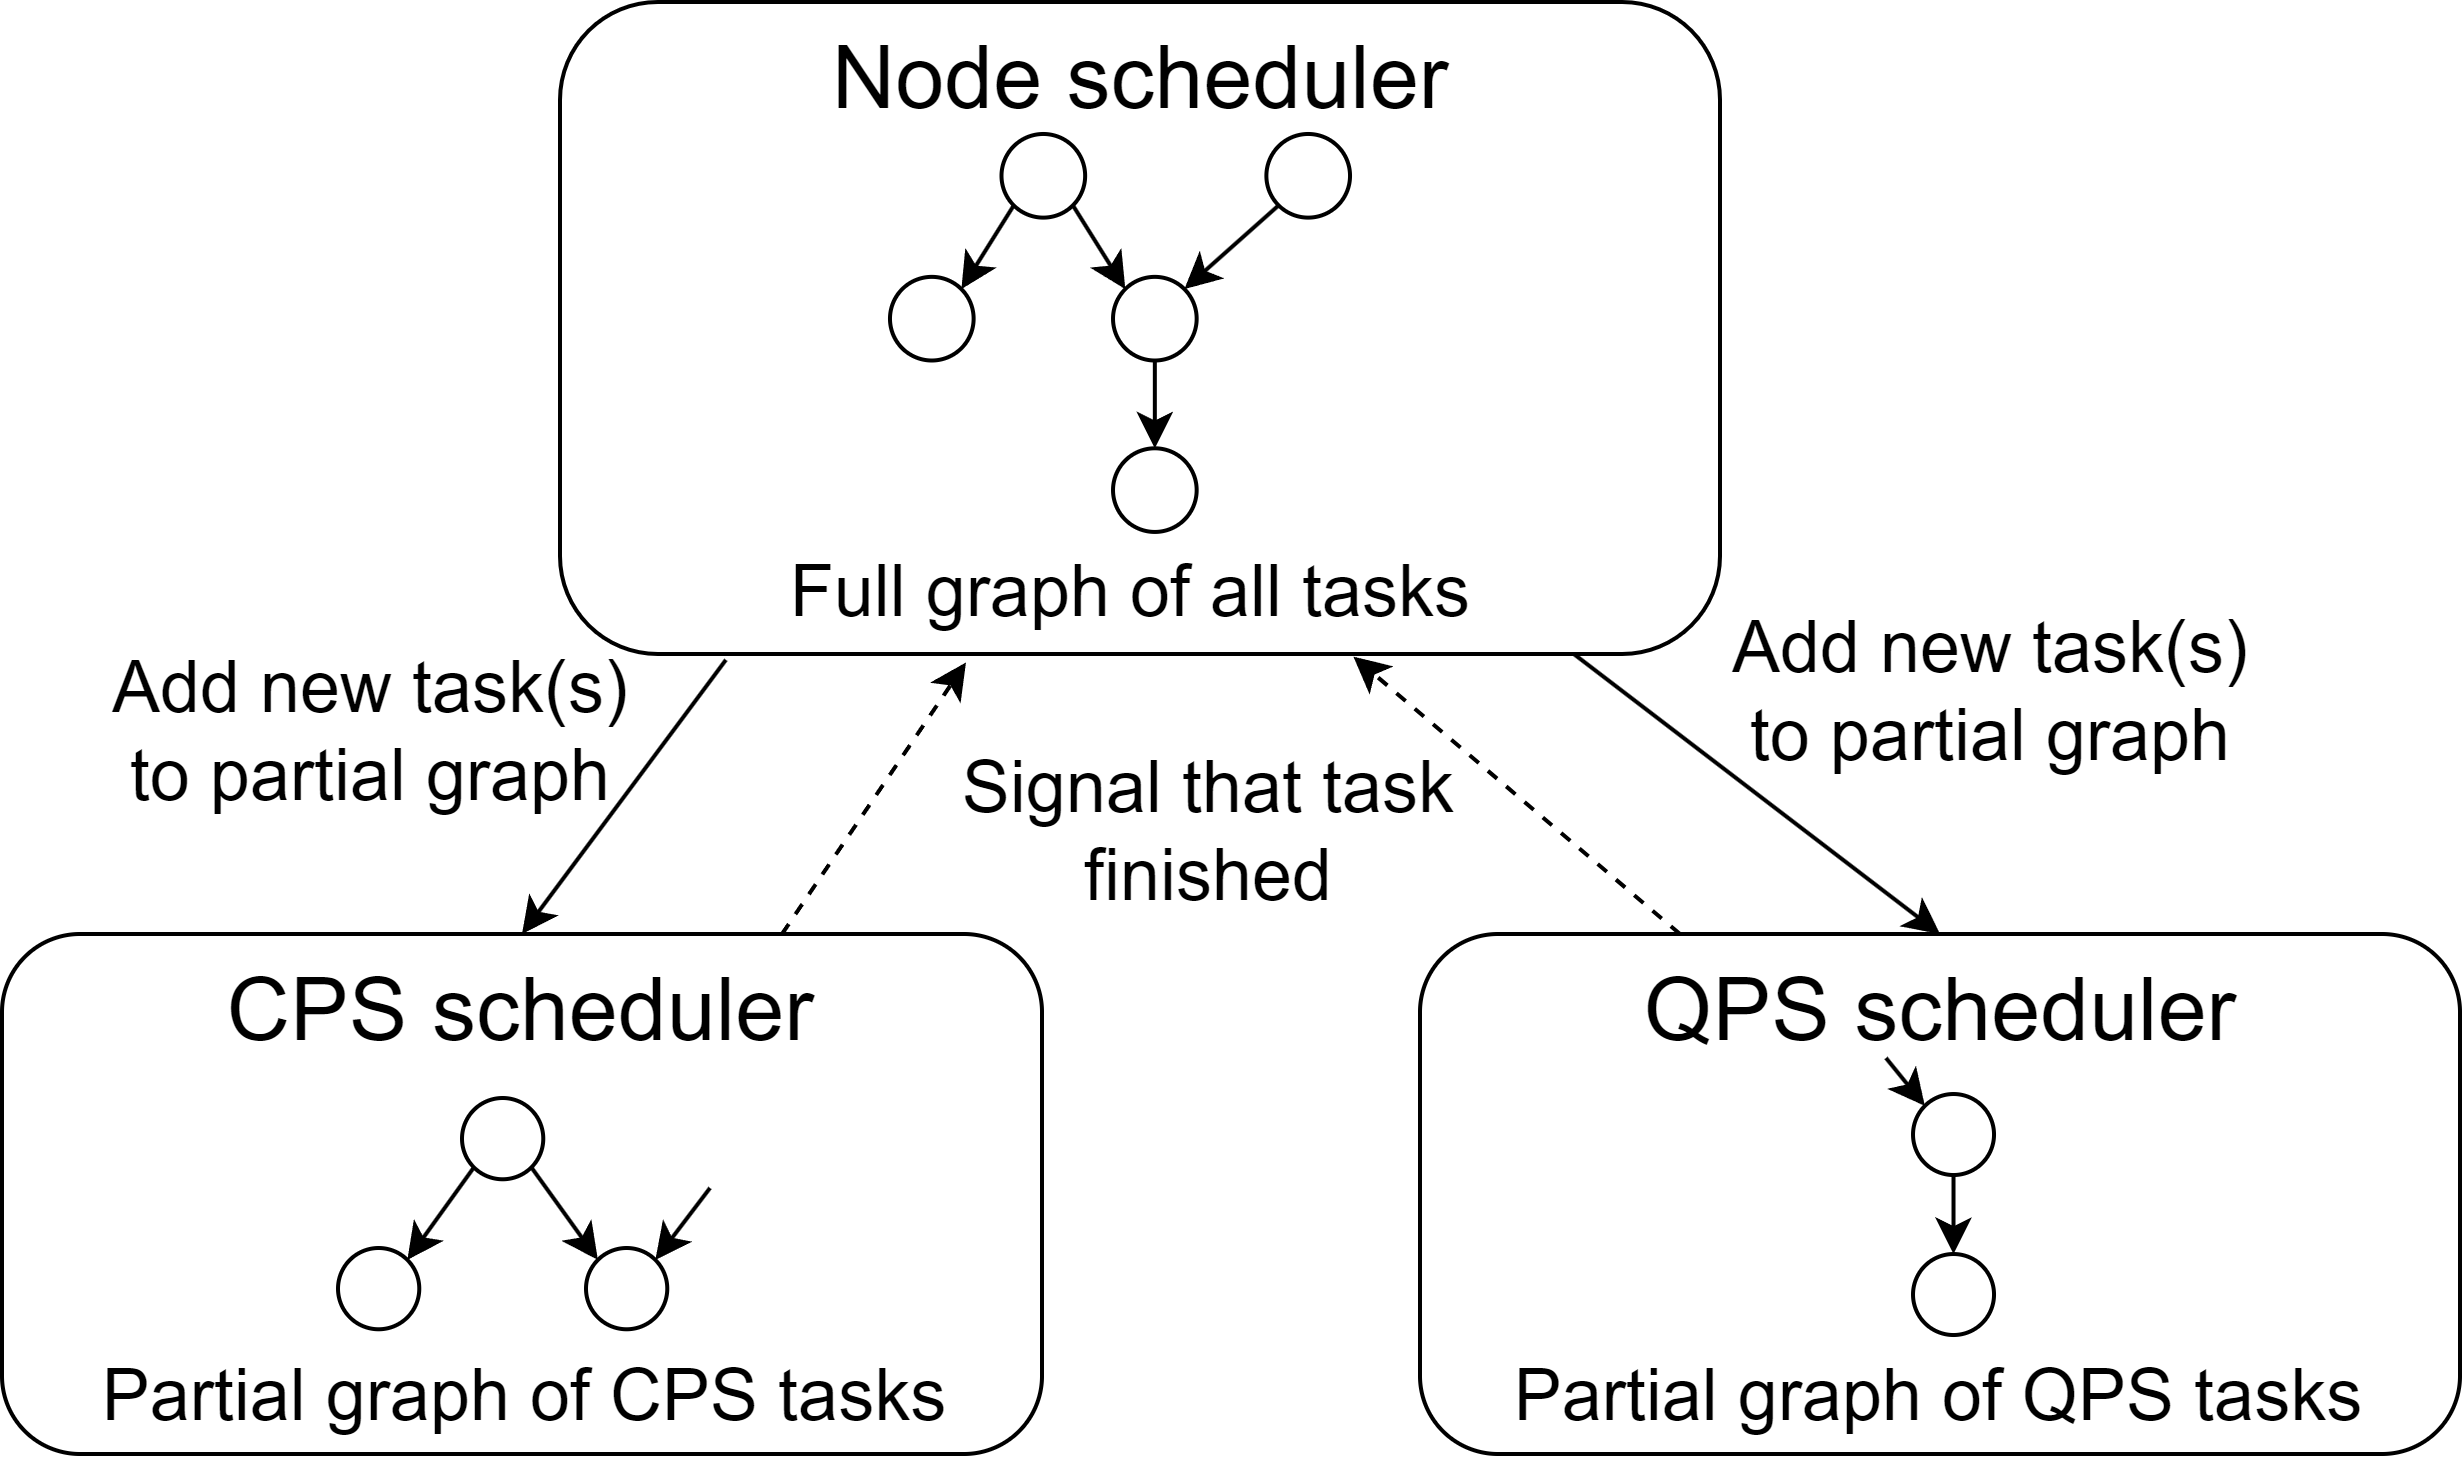
\includegraphics[width=\columnwidth]{figures/qoala/scheduler_components.png}
    \caption{Overview of our hierarchical scheduler implementation.
    The node scheduler maintains a graph of all tasks. The CPS and QPS maintain partial graphs with only tasks they can execute themselves. Partial graphs are updated by the node scheduler. 
    The CPS scheduler has access to a buffer with classical messages from other nodes, activating \texttt{HostEvent} tasks. The QPS scheduler has access to the network schedule, determining allowed start times of \texttt{Pair} tasks.}
    \label{qoala:fig:scheduler_impl}
\end{figure}




